\documentclass[tikz]{standalone}
\usepackage{pgfplots}
\usepackage{mathpazo}
\usepgfplotslibrary{polar}
\usepgflibrary{shapes.geometric}
\usetikzlibrary{calc}
\usetikzlibrary{datavisualization}
\usetikzlibrary{datavisualization.formats.functions}
\pgfplotsset{compat=1.12} 
\pgfplotsset{my style/.append style={axis x line=middle, axis y line=middle, xlabel={$x$},ylabel={$y$},smooth}}
%\tikzset{elegant/.style={smooth,thick,samples=50,cyan}}
%\tikzset{eaxis/.style={->,>=stealth}}
 
\begin{document}
\begin{tikzpicture}
	\begin{axis}[my style, xmin=-3.5,xmax=3.5,ymin=-0.02,ymax=0.45]
	\addplot[domain=-3:3]{1/sqrt(2*pi)*exp(-x^2/2)};
	\end{axis}
\end{tikzpicture}
\begin{tikzpicture}
	\begin{axis}[my style, xtick={-2,-1,0,1,2},xmin=-10,xmax=10,ymin=-10,ymax=10]
	%\addplot[domain=-3:5]{-abs(x-1)+3};
	%\addplot[domain=-7:1]{-x-2};
	\addplot[domain=-3:3]{exp(-x)*exp(-exp(-x))};
	%\addplot[domain=-3:3]{1/sqrt(2*pi)*exp(-x^2/2)};
	%\addplot[mark=*] coordinates{(1,-3)};
	%\addplot[mark=*,fill=white] coordinates{(1,1)};
	\end{axis}
\end{tikzpicture}
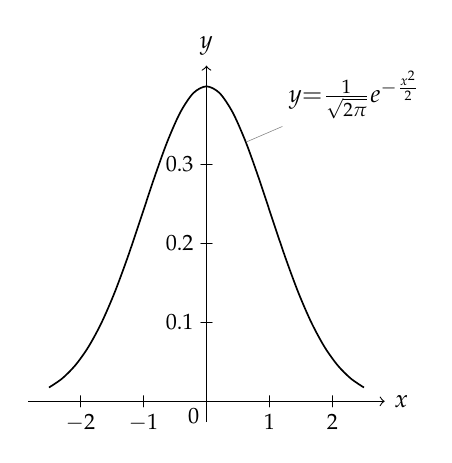
\begin{tikzpicture}[scale=1]
\datavisualization [school book axes, visualize as smooth line/.list={normal},all axes = {length=4cm,ticks = some},x axis ={label=$x$},y axis ={label=$y$},normal={pin in data={text=$y{=}\frac{1}{\sqrt{2\pi}}e^{-\frac{x^2}{2}}$,when=x is 0.5}}]
data [format=function] {
var x : interval [-2.5:2.5];
func y = 1/sqrt(2*pi)*exp(-(\value x)^2/2);
};
\end{tikzpicture}
 
\end{document}